\documentclass{amsart}
\usepackage{fullpage}

\usepackage[T1]{fontenc}
\usepackage[utf8]{inputenc} 
\usepackage{lmodern}
\usepackage[slovene]{babel}
\usepackage{hyperref}
\usepackage{amsmath,amssymb,amsfonts, mathtools}
\usepackage{graphicx}
\graphicspath{{./images/}}

\linespread{1.2}

\newcommand{\N}{\mathbb{N}}

% tekst napisan pokoncno
\theoremstyle{definition}
\newtheorem{definicija}{Definicija}[section]
\newtheorem{primer}[definicija]{Primer}
\newtheorem{opomba}[definicija]{Opomba}

\renewcommand\endprimer{\hfill$\diamondsuit$}

\theoremstyle{plain} % tekst napisan posevno
\newtheorem{lema}[definicija]{Lema}
\newtheorem{izrek}[definicija]{Izrek}
\newtheorem{trditev}[definicija]{Trditev}
\newtheorem{posledica}[definicija]{Posledica}

\newcommand\Vtextvisiblespace[1][.3em]{%
  \mbox{\kern.06em\vrule height.3ex}%
  \vbox{\hrule width#1}%
  \hbox{\vrule height.3ex}}

\title{Kontekstno-neodvisne gramatike za kodiranje in stiskanje podatkov}
\author{Janez Podlogar}
\date{\today}

\begin{document}

% \begin{abstract}

%     Placeholder

% \end{abstract}

\maketitle

\tableofcontents

\section{Kodiranje podatkov}

Zapis informacije v neki obliki ni primeren za vsakršno rabo. Besedilo, zapisano z pismenkami,
je neberljivo za slepe osebe, saj je komunikacijski kanal v tem primeru vid. Prav tako pisanega 
besedila v prvotni obliki ni mogoče poslati s telegrafom. V tem primeru je komunikacijski kanal
žica in pismenke se po njej ne morejo sprehoditi. V obeh primerih je informacija, ki bi jo radi 
prenesli, zapisana v neprimerni obliki. V prvem primeru je potrebno besedilo zapisati z Braillovo
pisavo. V drugem primeru pa je besedilo potrebno pretvoriti v električni signal. Spreminjanje 
zapisa sporočila imenujemo \textit{kodiranje}, sistemu pravil, po katerem se kodiranje opravi, pa
\textit{kod}.

\begin{primer}\label{Morse}

    \textit{Morsejeva abeceda} je kodiranje črk, števil in ločil s pomočjo zaporedja kratkih
    in dolgih signalov:

    \begin{itemize}
        \item Dolžina kratkega signala je ena enota.
        \item Dolgi signal je trikrat daljši od kratkega signala.
        \item Razmik med signali znotraj črke je tišina dolžine kratkega signala.
        \item Razmik med črkami je tišina dolga tri kratke signale oziroma en dolgi signal.
        \item Presledek med besedami je tišina dolga sedem kratkih signalov.
    \end{itemize}
 
    \begin{figure}[h]
        \centering
        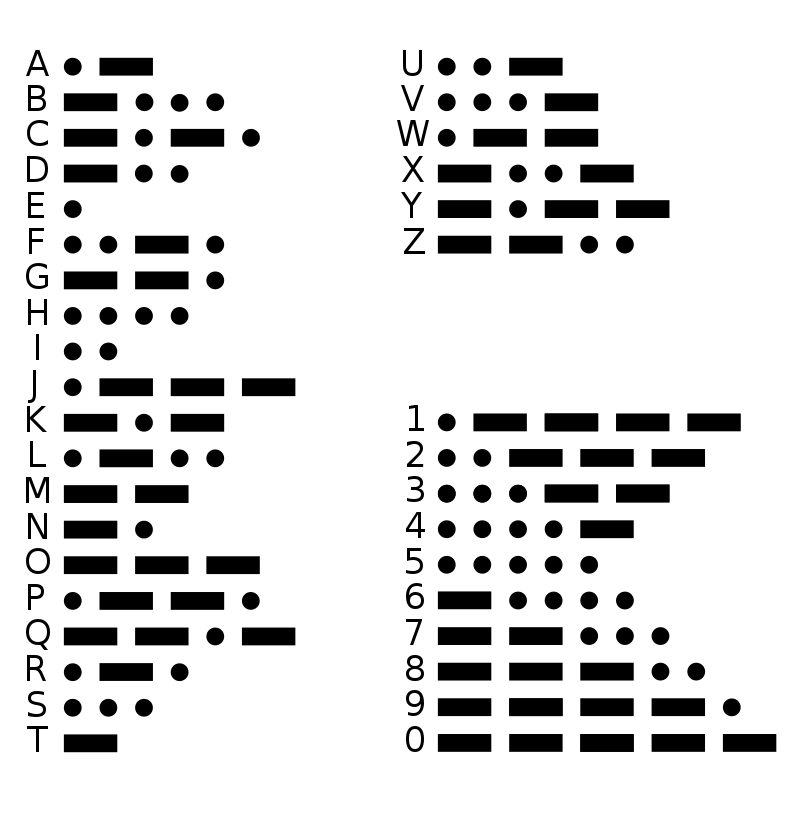
\includegraphics[width=4.3cm]{InternationalMorse.png}
        \caption{Mednarodna Morsejeva abeceda.}
        \label{fig:Morse}
    \end{figure}

    Prvotni namen Morsejeve abecede je komunikacija preko telegrama, saj komunikacijski
    kanal dovoljuje le električne signale in tišino med njimi. Kodiranje črk je takšno,
    da imajo črke z višjo frekvenco (v angleškem jeziku) krajši zapis. Tako se koda
    sporočila skrajša in posledično tudi čas njegovega prenosa.

\end{primer}

\begin{definicija}
    
    \textit{Abeceda} je končna neprazna množica. Elementom abecede pravimo \textit{črke}.
    Za abecedo $\Sigma$ definiramo
    \[
        \Sigma^0 = \{ \varepsilon \}
    \]
    in $\varepsilon$ imenujemo \textit{prazen niz}.
    Za vsak $ \ell > 0 $ rekurzivno definiramo \textit{množico vseh nizov abecede $\Sigma$
    dolžine $ \ell + 1 $}
    \[
        \Sigma^{\ell+1} = \{ wa \mid w \in \Sigma^{\ell} \text{ in } a \in \Sigma \}.
    \]
    Nadalnje, definiramo \textit{množica vseh končnih nizov abecede $\Sigma$}
    \[
        \Sigma^* = \bigcup_{\ell \geq 0} \Sigma^\ell
    \]
    in \textit{množica vseh končnih nizov abecede $\Sigma$ brez praznega niza}
    \[
        \Sigma^+ = \bigcup_{\ell > 0} \Sigma^\ell.
    \]
    \textit{Jezik na abecedi} $\Sigma$ je poljubna podmnožica množice $ \Sigma^* $.

\end{definicija}

\begin{definicija}
    
    Naj bo $\Sigma$ abeceda. Naj bo $*$ binarna operacija na množici vseh končnih nizov $ \Sigma^* $
    tako, da je prazen niz $\varepsilon$ nevtralni element in za niza $ w, u \in \Sigma^* $ velja
    \[
        w*u = w_1w_2 \cdots w_nu_1u_2 \cdots u_m,
    \]
    kjer sta $ w_1w_2 \cdots w_n $ in $ u_1u_2 \cdots u_m $ predstavitvi nizov $ w $ in $ u $ s 
    črkami abecede $ \Sigma $. Operacijo $*$ imneujemo \textit{stikanje} oziorma
    \textit{konkatenacija}. Znak $*$ spustimo in krajše pišemo $ wu $.
    
\end{definicija}

\begin{opomba}

    Stikanje je asociativna operacija. $ (\Sigma^*, *) $ je monoid in $ (\Sigma^+, *) $ je grupoid.

\end{opomba}

\begin{opomba}
    
    \textit{Kleenejeva zvezdica} oziroma \textit{Kleenejevo zaprtje} je enočlena operacija, ki 
    abecedi $\Sigma$ priredi najmanjšo nadmnožico $ \Sigma^* $, ki vsebuje \textit{prazen niz} 
    $\varepsilon$ in je zaprta za operacijo stikanje. Z drugimi besedami, $ \Sigma^* $ je množica
    vseh končnih nizov, ki jih lahko generiramo z stikanjem črk abecede $\Sigma$.
    
\end{opomba}

\begin{definicija}
    
    \textit{Dolžino niza w} označimo z $|w|$ in je enaka številu črk v nizu $ w \in \Sigma^* $.
    Natančneje, $ |w| = \ell $ natanko tedaj, ko je $ w \in \Sigma^\ell $. 

\end{definicija}

\begin{primer}
    
    Naj bo $ \Sigma = \{ a,b,c \} $ abeceda, potem so $ \mathit{ab} \in \Sigma^2, \mathit{ccc}
    \in \Sigma^3\text{ in } \mathit{cababcccababcccab} \in \Sigma^{17} $ končni nizi abecede
    $\Sigma$ in potemtakem elementi $ \Sigma^* $.

\end{primer}

\begin{definicija}
    
    \textit{Kodiranje nizov abecede} $\Sigma$ je injektivna funkcija $ \kappa \colon \Sigma^* \to
    \Sigma_c^* $, kjer je $ \Sigma_c^* $ neka abeceda, ki jo imenujemo $ \Sigma_c $
    \textit{kodna abeceda}, in $ \kappa(w) $ imenujemo \textit{koda niza} $ w $. 
    \textit{Dekodiranje kodiranja} $\kappa$ je funkcija  $ \delta \colon C \subseteq \Sigma^*_c 
    \to \Sigma^* $, da velja
    \[
        \forall w \in \Sigma^* \colon \delta(\kappa(w)) = w.
    \]

\end{definicija}

\begin{opomba}
    
    Funkcijo $ \kappa $ imenujemo \textit{kodna funkcija}, funkcijo $ \delta $ pa
    \textit{dekodna funckija}. 

\end{opomba}

\begin{opomba}
    
    Zožitev kodomene kodne funkcije $ \kappa $ na $ C \subseteq \Sigma^*_c $ je bijektivna funkcija.

\end{opomba}

\begin{primer}
    
    Formalizirajmo Morsejevo abecedo iz Primera~\refeq{Morse}. Abecedi sta
    \[
        \Sigma = \{ \text{A},  \text{B}, \ldots, \text{Z} \} \cup \{ 0, 1, \ldots, 9 \}
        \cup \{ \Vtextvisiblespace[5pt] \}, \quad
        \Sigma_c = \{ \cdot ,-, \Box \},
    \]
    kjer je \Vtextvisiblespace[5pt] presledek in $ \Box $ ena kratka enota tišine. Definirajmo kodno
    funkcijo črk abecede $ \kappa_s \colon \Sigma \to \Sigma_c^* $, ki vsaki črki iz abecede $ \Sigma_s $
    priredi niz črk kodne abecede $ \Sigma_c $. Predpis funkcije $ \kappa_s $ je določen s tabelo iz 
    Slike~\refeq{fig:Morse}, dodatno presledek \Vtextvisiblespace[5pt] kodiramo v tri kratkih enot tišine
    \[
        \kappa_s(\Vtextvisiblespace[5pt]) = \Box\Box\Box\Box.
    \]
    Za niz $ w = a_1a_2 \ldots a_n \in \Sigma^* $ definiramo kodno 
    funkcijo $ K $ po črkah
    \[
        \kappa(w) = \kappa_s(a_1) \Box\Box\Box \kappa_s(a_2) \Box\Box\Box \cdots \kappa_s(a_n).
    \]
    Poglejmo si dva primera kodiranja v Morsejevi abecedi
    \begin{gather*}
        \kappa(\text{SOS}) = \phantom{} \cdot\Box\cdot\Box\cdot \Box\Box\Box -\Box-\Box- \Box\Box\Box \cdot\Box\cdot\Box\cdot \phantom{}, \\
        \kappa(\text{AD\Vtextvisiblespace[5pt]HOC}) = \phantom{} \cdot\Box- \Box\Box\Box -\Box\cdot\Box\cdot 
        \Box\Box\Box\Box\Box\Box\Box
        \cdot\Box\cdot\Box\cdot\Box\cdot \Box\Box\Box -\Box-\Box- \Box\Box\Box -\Box\cdot\Box-\Box\cdot \phantom{}.
    \end{gather*}
    Recimo, da smo prejeli sporočilo, a se je pošiljatelj zmotil in je namesto kode,
    ki bi se dekodirala v
    \[
        \delta(\phantom{} -\Box-\Box\cdot\Box- \Box\Box\Box \cdot \Box\Box\Box -\Box\cdot\Box\cdot \phantom{}) = \text{QED},
    \]
    poslali kodo
    \[
        \phantom{} -\Box-\Box\cdot\Box-\Box- \Box\Box\Box \cdot \Box\Box\Box -\Box\cdot\Box\cdot \phantom{}.
    \]
    Sporočila ne znamo dekodirati, saj se ne nahaja v domeni $ C $ dekodne funkcije $ \delta $.

\end{primer}

\end{document}